\documentclass[tikz,border=5mm]{standalone}
\usepackage{tikz}
\usetikzlibrary{calc}

\begin{document}
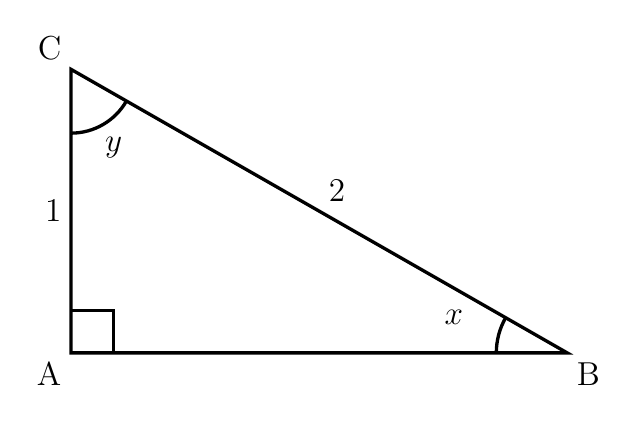
\begin{tikzpicture}[scale=1.8]

% Define vertices
\coordinate (C) at (0,2);
\coordinate (A) at (0,0);
\coordinate (B) at (3.5,0);

% Draw triangle CAB
\draw[very thick] (C) -- (A) -- (B) -- cycle;

% Draw right angle mark at A
\draw[very thick] (A) ++(0.3,0) -- ++(0,0.3) -- ++(-0.3,0);

% Calculate angle from C to B
\pgfmathsetmacro{\angleCtoA}{-90}
\pgfmathsetmacro{\angleCtoB}{atan2(-2, 3.5)}

% Angle arc at C (y) - inside
\def\arcRadC{0.45}
\draw[very thick] ($(C)+({\angleCtoA}:\arcRadC)$) arc[start angle=\angleCtoA, end angle=\angleCtoB, radius=\arcRadC];
\node at ($(C)+(0.3,-0.55)$) {\large $y$};

% Calculate angle from B to C
\pgfmathsetmacro{\angleBtoA}{180}
\pgfmathsetmacro{\angleBtoC}{atan2(2, -3.5)}

% Angle arc at B (x) - inside
\def\arcRadB{0.5}
\draw[very thick] ($(B)+({\angleBtoC}:\arcRadB)$) arc[start angle=\angleBtoC, end angle=\angleBtoA, radius=\arcRadB];
\node at ($(B)+(-0.8,0.25)$) {\large $x$};

% Vertex labels
\node[above left] at (C) {\large C};
\node[below left] at (A) {\large A};
\node[below right] at (B) {\large B};

% Side labels
\node[left] at ($(C)!0.5!(A)$) {\large $1$};
\node[above right] at ($(C)!0.5!(B)$) {\large $2$};

\end{tikzpicture}
\end{document}